

\begin{figure}[h!]
\centering
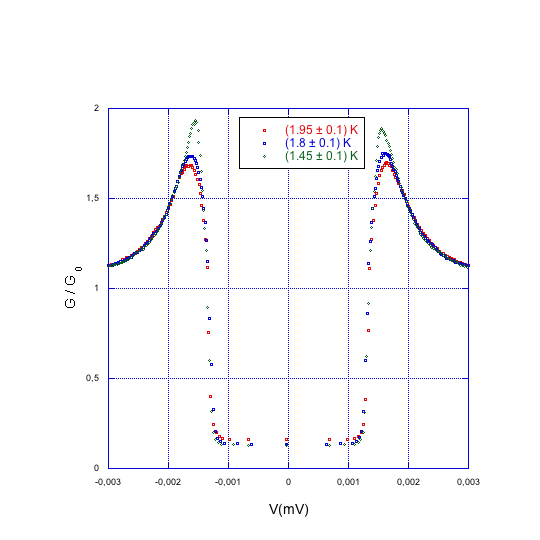
\includegraphics[scale=0.4]{graph1}
\caption{Hola\label{graph1}}
\end{figure}

\begin{figure}[h!]
\centering
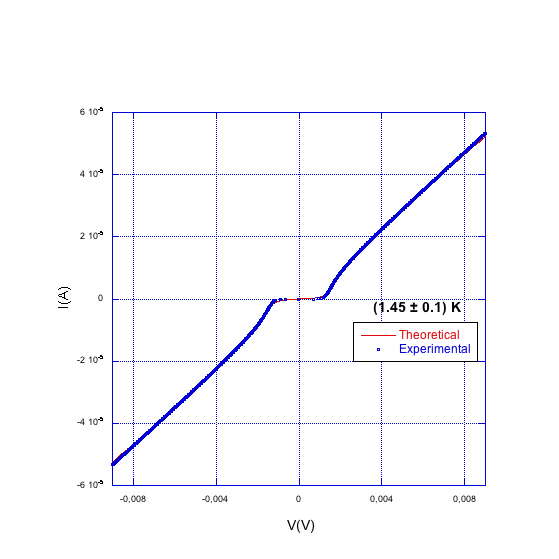
\includegraphics[scale=0.4]{graph2}
\caption{Hola\label{graph2}}
\end{figure}

\begin{figure}[h!]
\centering
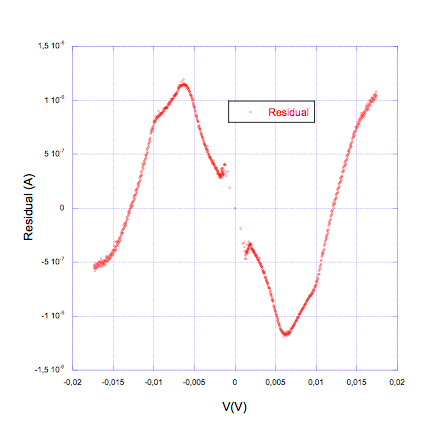
\includegraphics[scale=0.4]{graph3}
\caption{Hola\label{graph3}}
\end{figure}

\begin{figure}[h!]
\centering
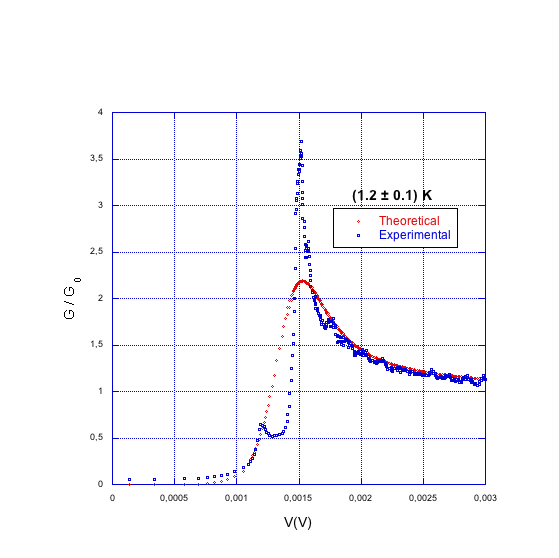
\includegraphics[scale=0.4]{graph4}
\caption{Hola\label{graph4}}
\end{figure}

\begin{figure}[h!]
\centering
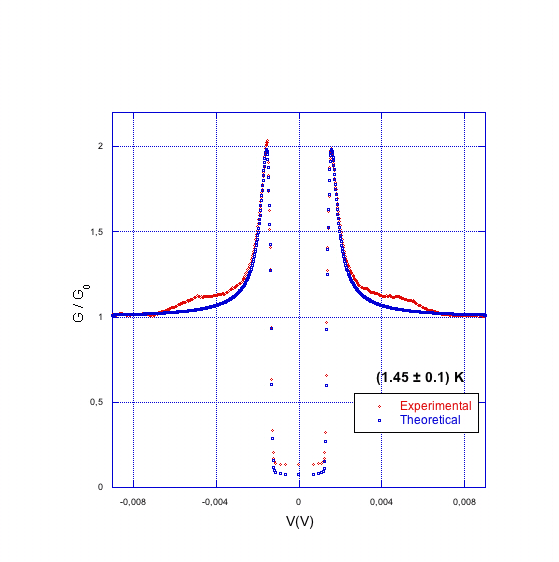
\includegraphics[scale=0.4]{graph5}
\caption{Hola\label{graph5}}
\end{figure}



1) Levenberg-Marquard??? The best method: by hand... :-)
2) Graphs: commentary on ALL the characteristics...
3) BCS is not totally correct --> real density of states is not the BCS's one, phonons,
4) ...


These are the Experimental ResultsThese are the Experimental Results These are the Experimental Results These are the Experimental Results These are the Experimental Results These are the Experimental Results These are the Experimental Results These are the Experimental Results These are the Experimental Results These are the Experimental Results These are the Experimental Results These are the Experimental Results These are the Experimental Results These are the Experimental Results These are the Experimental Results These are the Experimental Results These are the Experimental Results These are the Experimental Results These are the Experimental Results These are the Experimental Results These are the Experimental Results 